\chapter{Νευρωνικά δίκτυα}
\label{chapter2}
\graphicspath{{./images/deep-learning-in-cardiology/}}

\newcommand{\networkLayer}[6]{
	\def\a{#1}
	\def\b{0.02}
	\def\c{#2}
	\def\t{#3}
	\def\d{#4}
	\draw[line width=0.3mm] (\c+\t,0,\d) -- (\c+\t,\a,\d) -- (\t,\a,\d);                                                      % back plane
	\draw[line width=0.3mm] (\t,0,\a+\d) -- (\c+\t,0,\a+\d) node[midway,below] {#6} -- (\c+\t,\a,\a+\d) -- (\t,\a,\a+\d) -- (\t,0,\a+\d); % front plane
	\draw[line width=0.3mm] (\c+\t,0,\d) -- (\c+\t,0,\a+\d);
	\draw[line width=0.3mm] (\c+\t,\a,\d) -- (\c+\t,\a,\a+\d);
	\draw[line width=0.3mm] (\t,\a,\d) -- (\t,\a,\a+\d);
	\filldraw[#5] (\t+\b,\b,\a+\d) -- (\c+\t-\b,\b,\a+\d) -- (\c+\t-\b,\a-\b,\a+\d) -- (\t+\b,\a-\b,\a+\d) -- (\t+\b,\b,\a+\d); % front plane
	\filldraw[#5] (\t+\b,\a,\a-\b+\d) -- (\c+\t-\b,\a,\a-\b+\d) -- (\c+\t-\b,\a,\b+\d) -- (\t+\b,\a,\b+\d);
	\ifthenelse {\equal{#5} {}}
	{}
	{\filldraw[#5] (\c+\t,\b,\a-\b+\d) -- (\c+\t,\b,\b+\d) -- (\c+\t,\a-\b,\b+\d) -- (\c+\t,\a-\b,\a-\b+\d);} % Else, draw a colored slice.
}

\section{Εισαγωγή}
Η μηχανική μάθηση είναι ένα σύνολο μεθόδων Τεχνητής Νοημοσύνης (Artificial Intelligence, AI) που επιτρέπει στους υπολογιστές να μαθαίνουν μια διαδικασία χρησιμοποιώντας δεδομένα, αντί να προγραμματιστούν ρητά.
Έχει αναδειχθεί ως ένας αποτελεσματικός τρόπος χρήσης και συνδυασμού βιολογικών δεικτών, απεικόνισης, συσσωρευμένης κλινικής έρευνας από τη βιβλιογραφία και τους Ηλεκτρονικούς Φακέλους Υγείας (Electronic Health Record, EHR) για την αύξηση της ακρίβειας λύσεων ενός ευρύ φάσματος ιατρικών προβλημάτων.
Οι ιατρικές διαδικασίες που χρησιμοποιούν την μηχανική μάθηση εξελίσσονται από τέχνη σε επιστήμη με γνώμονα τα δεδομένα, προσφέροντας διόραση από τα πληθυσμιακά δεδομένα στην προσωποποιημένη ιατρική.

Η βαθιά μάθηση, και η εφαρμογή της στα νευρωνικά δίκτυα τα Βαθιά Νευρωνικά Δίκτυα (Deep Neural Networks, DNN), είναι ένα σύνολο μεθόδων μηχανικής μάθησης που αποτελούνται από πολλαπλά στοιβαγμένα επίπεδα και χρησιμοποιούν δεδομένα για να μάθουν ιεραρχικά επίπεδα.
Η βαθιά μάθηση προέκυψε λόγω της αύξησης της υπολογιστικής ισχύος των μονάδων επεξεργασίας γραφικών και της διαθεσιμότητας δεδομένων μεγάλου όγκου και έχει αποδειχθεί ότι είναι μια ισχυρή λύση για προβλήματα όπως ταξινόμηση εικόνων~\cite{krizhevsky2012imagenet}, κατάτμηση εικόνας~\cite{ronneberger2015u}, επεξεργασία φυσικής γλώσσας~\cite{collobert2008unified}, αναγνώριση ομιλίας~\cite{graves2013speech} και γονιδιωματική~\cite{alipanahi2015predicting}.

Πλεονεκτήματα των DNN έναντι των παραδοσιακών τεχνικών μηχανικής μάθησης περιλαμβάνουν ότι απαιτούν λιγότερη εξειδικευμένη γνώση για το πρόβλημα που προσπαθούν να λύσουν και επίσης είναι ευκολότερο να αυξήσουν την ακρίβεια τους είτε με την αύξηση του συνόλου δεδομένων εκπαίδευσης ή την αύξηση της χωρητικότητας του δικτύου.
Τα ρηχά μοντέλα μηχανικής μάθησης, όπως τα δέντρα αποφάσεων και οι Μηχανές Διανυσμάτων Υποστήριξης (Support Vector Machines, SVM), είναι `ανεπαρκή'; το οποίο σημαίνει ότι απαιτούν μεγάλο αριθμό υπολογισμών κατά τη διάρκεια της εκπαίδευσης/συμπερασμού, μεγάλο αριθμό παρατηρήσεων για την επίτευξη γενίκευσης και σημαντική ανθρώπινη εργασία για τον προσδιορισμό της πρότερης γνώσης του μοντέλου~\cite{bengio2007scaling}.

\section{Επισκόπηση θεωρίας}
Τα νευρωνικά δίκτυα είναι ένα σύνολο τεχνικών μηχανικής μάθησης εμπνευσμένων από τον εγκέφαλο αλλά χωρίς πρωταρχικό στόχο να τον προσομοιώνουν.
Πρόκειται για μεθόδους προσέγγισης συναρτήσεων όπου η είσοδος $\mathbf{x}$ μπορεί να είναι κείμενο, εικόνα, ήχος, σήμα, τρισδιάστατος όγκος, βίντεο (ή συνδυασμός αυτών) και η έξοδος $\mathbf{y}$ είναι από το ίδιο σετ με το $\mathbf{x}$ αλλά αυξημένου ενημερωτικού περιεχομένου.
Με μαθηματικούς όρους, ο στόχος ενός νευρωνικού δικτύου είναι να βρει το σύνολο παραμέτρων $\theta$ (το οποίο αποτελείται από βάρη $\mathbf{w}$ και πολώσεις $\mathbf{b}$):
\begin{equation}
	\centering
	f(\mathbf{x};\mathbf{\theta}) = \mathbf{\hat{y}}
\end{equation}

\noindent
όπου $f$ είναι μια προκαθορισμένη συνάρτηση και $\mathbf{\hat{y}}$ είναι η πρόβλεψη.
Ο περιορισμός για το $\theta$ είναι να έχουμε ένα όσο το δυνατόν χαμηλότερη τιμή για μια συνάρτηση κόστους $J(\theta)$ μεταξύ του $\mathbf{y}$ και του $\mathbf{\hat{y}}$.

Η βασική μονάδα των νευρωνικών δικτύων είναι ο αντιλήπτωρ που απεικονίζεται στην Εικ.\ref{fig:perceptron}, ο οποίος δημοσιεύθηκε για πρώτη φορά από τον Rosenblatt~\cite{rosenblatt1958perceptron} το 1958.
Αποτελείται από ένα σύνολο εισόδων που συμβολίζεται με το διάνυσμα $\mathbf{x}=[x_1, \ldots, x_j, \ldots, x_n]$, ένα σύνολο βαρών για την κάθε είσοδο, που συμβολίζεται με το διάνυσμα $\mathbf{w}=[w_1, \ldots, w_j, \ldots, w_n]$ και η πόλωση $b$.
Η απόφαση του κόμβου να πυροδοτήσει ένα σήμα $\alpha$ στον επόμενο νευρώνα ή στην έξοδο καθορίζεται από τη συνάρτηση ενεργοποίησης $\phi$, το σταθμισμένο άθροισμα $\mathbf{w}$ και τη πόλωση $b$, με τον ακόλουθο τρόπο:
\begin{equation}
	\centering
	\alpha = \phi(\sum\limits_{j} w_{j}x_{j} + b)
\end{equation}

Οι τιμές του διανύσματος βαρών $\mathbf{w}$ και των πολώσεων $\mathbf{b}$ στα DNN ρυθμίζονται επαναληπτικά χρησιμοποιώντας αλγόριθμους βελτιστοποίησης που βασίζονται στην κλίση καθόδου και την αντίστροφη διάδοση σφάλματος (backpropagation)~\cite{rumelhart1986learning} ο οποίος υπολογίζει την κλίση της συνάρτησης κόστους σε σχέση με τις παραμέτρους $\nabla_{\theta}J(\theta)$~\cite{goodfellow2016deep}.
Η αξιολόγηση της γενίκευσης ενός νευρωνικού δικτύου απαιτεί τη διάσπαση του αρχικού συνόλου δεδομένων $D=(\mathbf{x}, \mathbf{y})$ σε τρία μη-αλληλεπικαλυπτόμενα σύνολα δεδομένων:
\begin{equation}
	\centering
	D_{train}=(\mathbf{x}_{train}, \mathbf{y}_{train})
\end{equation}

\begin{equation}
	\centering
	D_{validation}=(\mathbf{x}_{validation}, \mathbf{y}_{validation})
\end{equation}

\begin{equation}
	\centering
	D_{test}=(\mathbf{x}_{test}, \mathbf{y}_{test})
\end{equation}


Το $D_{train}$ χρησιμοποιείται για την μάθηση των $\mathbf{w}$ και $\mathbf{b}$, των οποίων οι τιμές κάνουν το δίκτυο να ελαχιστοποιεί την επιλεγμένη συνάρτηση κόστους, ενώ το $D_{validation}$ χρησιμοποιείται για την επιλογή των υπερπαραμέτρων του δικτύου.
Το $D_{test}$ χρησιμοποιείται για την αξιολόγηση της γενίκευσης του δικτύου και θα πρέπει ιδανικά να προέρχεται από διαφορετικές μηχανές/ασθενείς/οργανισμούς ανάλογα με το ερευνητικό ερώτημα.

\begin{figure}[!t]
	\centering
	\begin{tikzpicture}[]
	\node[circle, draw=white] (x1) at (0, 4) {$x_1$};
	\node at (0, 3) {$\vdots$};
	\node[circle, draw=white] (xj) at (0, 2) {$x_j$};
	\node at (0, 1) {$\vdots$};
	\node[circle, draw=white] (xn) at (0, 0) {$x_n$};
	\node[circle, draw=white] (b) at (4, 4) {$b$};
	\node[circle, draw=black] (sigma) at (4, 2) {$\phi$};
	\node[circle, draw=white] (output) at (6, 2) {$\alpha$};
	\draw[->] (x1) to node[above]{$w_1$} (sigma);
	\draw[->] (xj) to node[above]{$w_j$} (sigma);
	\draw[->] (xn) to node[above]{$w_n$} (sigma);
	\draw[->] (b) -- (sigma);
	\draw[->] (sigma) -- (output);
\end{tikzpicture}

	\caption[Αντιλήπτωρ]{Αντιλήπτωρ.
	Περιέχει ένα σύνολο συνδέσεων $x_{1, \ldots, n}$ ως εισόδους, τα βάρη $w_{1, \ldots, n}$, τη πόλωση $b$, τη συνάρτηση ενεργοποίησης $\phi$ και την έξοδο $\alpha$.
	}
	\label{fig:perceptron}
\end{figure}

Η απόδοση των DNN έχει βελτιωθεί σημαντικά με τη χρήση της ανορθωμένης γραμμικής μονάδας (Rectified Linear Unit, ReLU) ως συνάρτηση ενεργοποίησης σε σύγκριση με την σιγμοειδής και την υπερβολική εφαπτομένη~\cite{glorot2011deep}.
Η συνάρτηση ενεργοποίησης του τελευταίου επιπέδου επιλέγεται με βάση τη φύση του ερευνητικού ερωτήματος που πρέπει να απαντηθεί (π.χ.\ softmax για ταξινόμηση, σιγμοειδής για παλινδρόμηση).

Οι συναρτήσεις κόστους που χρησιμοποιούνται στα νευρωνικά δίκτυα εξαρτώνται επίσης από το πρόβλημα που πρέπει να επιλυθεί.
Η διασταυρωμένη εντροπία (cross-entropy) ποσοτικοποιεί τη διαφορά μεταξύ της πραγματικής και της προβλεπόμενης κατανομής πιθανοτήτων και επιλέγεται συνήθως για προβλήματα ανίχνευσης και ταξινόμησης.
Το εμβαδόν της περιοχής κάτω από την καμπύλη λειτουργίας δέκτη (Area Under Curve, AUC) αντιπροσωπεύει την πιθανότητα ένα τυχαίο ζεύγος κανονικών και μη κανονικών εικονοστοιχείων/σημάτων/εικόνων να ταξινομηθεί σωστά~\cite{hanley1982meaning} και χρησιμοποιείται σε προβλήματα δυαδικής τμηματοποίησης.
Ο συντελεστής Dice~\cite{dice1945measures} είναι ένα μέτρο ομοιότητας που χρησιμοποιείται στα προβλήματα τμηματοποίησης και οι τιμές του κυμαίνονται μεταξύ μηδέν (συνολική αναντιστοιχία) και μονάδας (τέλεια αντιστοίχιση).

\section{Επισκόπηση αρχιτεκτονικών}
Τα Πλήρως Συνδεδεμένα Δίκτυα (Fully Connected Networks, FNN) είναι δίκτυα που αποτελούνται από πολλαπλούς αντιλήπτωρες στοιβαγμένους σε πλάτος και βάθος, που σημαίνει ότι κάθε αντιλήπτωρ σε κάθε επίπεδο συνδέεται με κάθε αντιλήπτωρ στα επίπεδα αμέσως πριν και μετά.
Αν και έχει αποδειχθεί~\cite{hornik1989multilayer} ότι τα FNN ενός επιπέδου με επαρκή αριθμό κρυφών μονάδων είναι καθολικοί προσεγγιστές συναρτήσεων, δεν είναι υπολογιστικά αποδοτικά για την προσέγγιση σύνθετων συναρτήσεων.
Τα Δίκτυα Βαθιάς Πίστης (Deep Belief Networks, DBN)~\cite{hinton2006fast} είναι στοιβαγμένες Περιορισμένες Μηχανές Boltzmann (Restricted Boltzmann Machines, RBMs) όπου κάθε επίπεδο κωδικοποιεί τις στατιστικές εξαρτήσεις μεταξύ των μονάδων στο προηγούμενο επίπεδο; εκπαιδεύονται για να μεγιστοποιήσουν την πιθανοφάνεια των δεδομένων εκπαίδευσης.

Τα Συνελικτικά Νευρωνικά Δίκτυα (Convolutional Neural Networks, CNN), όπως φαίνεται στο Σχήμα~\ref{fig:cnn}, αποτελούνται από ένα συνελικτικό μέρος στο οποίο γίνεται ιεραρχική εξαγωγή χαρακτηριστικών (χαρακτηριστικά χαμηλού επιπέδου όπως ακμές και γωνίες και χαρακτηριστικά υψηλού επιπέδου, όπως τμήματα αντικειμένων) και ένα πλήρως συνδεδεμένο μέρος για ταξινόμηση ή παλινδρόμηση, ανάλογα με τη φύση της εξόδου $y$.
Τα συνελικτικά επίπεδα είναι πολύ καλοί βελτιστοποιητές χαρακτηριστικών που χρησιμοποιούν τις τοπικές σχέσεις των δεδομένων, ενώ τα πλήρως συνδεδεμένα επίπεδα είναι καλοί ταξινομητές, επομένως χρησιμοποιούνται ως τα τελευταία επίπεδα ενός CNN\@.
Επιπλέον, τα συνελικτικά επίπεδα δημιουργούν χάρτες ενεργοποιήσεων χρησιμοποιώντας κοινόχρηστα βάρη που έχουν σταθερό αριθμό παραμέτρων σε αντίθεση με τα πλήρως συνδεδεμένα επίπεδα, καθιστώντας τα έτσι πολύ ταχύτερα.
Το VGGnet~\cite{simonyan2014very} είναι μια απλή CNN αρχιτεκτονική που χρησιμοποιεί μικρά συνελικτικά φίλτρα ($3\times 3$) και η απόδοση του αυξάνεται απλά αυξάνοντας το βάθος του δικτύου.
Το GoogleNet~\cite{szegedy2015going} είναι μια άλλη CNN αρχιτεκτονική η οποία χρησιμοποιεί την μονάδα inception.
Η μονάδα inception χρησιμοποιεί παράλληλα πολλαπλά επίπεδα περιελίξεων από τα οποία το αποτέλεσμα συσσωρεύεται σειριακά, επιτρέποντας έτσι στο δίκτυο να μαθαίνει χαρακτηριστικά πολλαπλών επιπέδων.
Το ResNet~\cite{he2016deep} είναι μια CNN αρχιτεκτονική η οποία διαμορφώνει τα επίπεδα ως συναρτήσεις μάθησης υπολειμμάτων με βάση τις εισόδους των επιπέδων, επιτρέποντας την δημιουργία πολύ πιο βαθιών δικτύων, σε σχέση με τα προηγουμένως αναφερθέντα.

\begin{figure}[!t]
	\centering
	\begin{tikzpicture}[scale=0.9]
	\draw[dashed] (0.03, 0) -- (1.5, 0);
	\draw[dashed] (1.61, 0) -- (3.01, 0);
	\draw[dashed] (3.2, 0) -- (4.5, 0);
	\draw[dashed] (4.9, 0) -- (6, 0);
	\draw[dashed] (6.8, 0) -- (7.5, 0);
	\networkLayer{4.0}{0.03}{0}{0.0}{color=white}{}
	\networkLayer{3.5}{0.1}{1.5}{0.0}{color=white}{}
	\networkLayer{3.0}{0.2}{3.0}{0.0}{color=white}{}
	\networkLayer{2.5}{0.4}{4.5}{0.0}{color=white}{}
	\networkLayer{2.0}{0.8}{6.0}{0.0}{color=white}{}
	\networkLayer{1.5}{1.6}{7.5}{0.0}{color=white}{}
	\draw[dashed] (10, -1) -- (11.5, 0.5);
	\draw[-] (10.5, -1) -- (12, 0.5);
	\draw[-] (10.5, -0.5) -- (12, 1);
	\draw[-] (10, -0.5) -- (11.5, 1);
	\draw[-] (12, 1) -- (11.5, 1);
	\draw[-] (12, 1) -- (12, 0.5);
	\draw[-] (10, -1) rectangle ++ (0.5,0.5) node{};
	\node[canvas is zy plane at x=0, scale=0.9] at (-0.735, 1.235){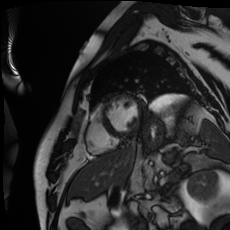
\includegraphics[scale=0.491]{mri_image.png}};
	\node[canvas is zy plane at x=0, scale=0.9] at (0.93, 1.07){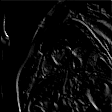
\includegraphics[scale=0.89]{layer_0_feature_map_0.png}};
	\node[canvas is zy plane at x=0, scale=0.9] at (0.83, 1.07){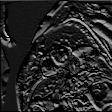
\includegraphics[scale=0.89]{layer_0_feature_map_2.png}};
	\node[canvas is zy plane at x=0, scale=0.9] at (2.63, 0.93){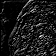
\includegraphics[scale=1.52]{layer_1_feature_map_0.png}};
	\node[canvas is zy plane at x=0, scale=0.9] at (2.42, 0.93){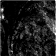
\includegraphics[scale=1.52]{layer_1_feature_map_1.png}};
	\node[canvas is zy plane at x=0, scale=0.9] at (4.42, 0.78){
\includegraphics[scale=2.53]{layer_2_feature_map_0.png}};
	\node[canvas is zy plane at x=0, scale=0.9] at (4.03, 0.78){
\includegraphics[scale=2.53]{layer_2_feature_map_3.png}};
	\node[canvas is zy plane at x=0, scale=0.9] at (6.42, 0.611){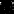
\includegraphics[scale=4.05]{layer_3_feature_map_0.png}};
	\node[canvas is zy plane at x=0, scale=0.9] at (5.6, 0.611){
\includegraphics[scale=4.05]{layer_3_feature_map_2.png}};
	\node[canvas is zy plane at x=0, scale=0.9] at (8.815, 0.472){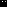
\includegraphics[scale=6.05]{layer_4_feature_map_0.png}};
	\node[canvas is zy plane at x=0, scale=0.9] at (7.22, 0.472){
\includegraphics[scale=6.05]{layer_4_feature_map_1.png}};
	\node at (8, 0.472) {$\dots$};
	\node at (6, 0.472) {$\dots$};
	\node[canvas is zy plane at x=0] at (-1, -3){
\includegraphics[scale=10]{layer_4_filter_0.png}};
	\node at (-0.8, -3) {$\dots$};
	\node[canvas is zy plane at x=0] at (-0.6, -3){
\includegraphics[scale=10]{layer_4_filter_1.png}};
	\node[canvas is zy plane at x=0] at (0.8, -3){
\includegraphics[scale=10]{layer_9_filter_0.png}};
	\node at (1, -3) {$\dots$};
	\node[canvas is zy plane at x=0] at (1.3, -3){
\includegraphics[scale=10]{layer_9_filter_1.png}};
	\node[canvas is zy plane at x=0] at (2.5, -3){
\includegraphics[scale=10]{layer_16_filter_0.png}};
	\node at (2.7, -3) {$\dots$};
	\node[canvas is zy plane at x=0] at (2.9, -3){
\includegraphics[scale=10]{layer_16_filter_1.png}};
	\node[canvas is zy plane at x=0] at (4.2, -3){
\includegraphics[scale=10]{layer_23_filter_0.png}};
	\node at (4.4, -3) {$\dots$};
	\node[canvas is zy plane at x=0] at (4.6, -3){
\includegraphics[scale=10]{layer_23_filter_1.png}};
	\node[canvas is zy plane at x=0] at (6.3, -3){
\includegraphics[scale=10]{layer_30_filter_0.png}};
	\node at (6.5, -3) {$\dots$};
	\node[canvas is zy plane at x=0] at (6.7, -3){
\includegraphics[scale=10]{layer_30_filter_1.png}};
	\draw[<-] (-0.3, -3) -- (0.3, -3);
	\draw[<-] (1.6, -3) -- (2.1, -3);
	\draw[<-] (3.2, -3) -- (3.9, -3);
	\draw[<-] (4.8, -3) -- (5.9, -3);
	\draw[<-] (7.1, -3) -- (13.0, -3);
	\draw[dashed] (-1.51, -1.53) -- (0.15, -1.35);
	\draw[dashed] (0.27, -1.35) -- (1.85, -1.16);
	\draw[dashed] (2.05, -1.16) -- (3.55, -0.97);
	\draw[dashed] (3.95, -0.97) -- (5.25, -0.77);
	\draw[dashed] (6.02, -0.78) -- (6.94, -0.57);
	\draw[dashed] (-1.51, 2.45) -- (0.15, 2.15);
	\draw[dashed] (0.27, 2.15) -- (1.85, 1.85);
	\draw[dashed] (2.05, 1.85) -- (3.55, 1.54);
	\draw[dashed] (3.95, 1.54) -- (5.25, 1.23);
	\draw[dashed] (6.02, 1.22) -- (6.94, 0.91);
	\draw[dashed] (0.03, 4) -- (1.5, 3.51);
	\draw[dashed] (1.61, 3.51) -- (3.01, 3.01);
	\draw[dashed] (3.2, 3) -- (4.5, 2.5);
	\draw[dashed] (4.9, 2.51) -- (6, 2);
	\draw[dashed] (6.8, 2) -- (7.5, 1.5);
	\draw[dotted] (9.1, 1.5) --(11.5, 1);
	\draw[dotted] (9.1, 0) -- (11.5, 0.5);
	\draw[dotted] (8.5, 0.92) -- (10, -0.5);
	\draw[dotted] (8.5, -0.58) --  (10, -1);
	\draw[dashdotted] (10.5, -0.5) -- (13, -0.25);
	\draw[dashdotted] (10.5, -1) -- (13, -0.25);
	\draw[dashdotted] (12, 1) -- (13, -0.25);
	\draw[dashdotted] (12, 0.5) -- (13, -0.25);
	\node[align=left] at (13.3,-0.2) {$\hat{y}$};
	\draw[->] (13.3, -0.6) -- (13.3, -2.7) node [pos=1.1] {$J$};
	\draw[<-] (13.5, -3) -- (14, -3) node [pos=1.6] {$y$};
	\node[align=left] at (10.0, -2.4) {αντίστροφη διάδοση σφάλματος};
	\node[align=left] at (10.8, 2.5) {προς-τα-εμπρός διάδοση};
\end{tikzpicture}

	\caption[Συνελικτικό νευρωνικό δίκτυο]{Ένα συνελικτικό νευρωνικό δίκτυο που υπολογίζει την εμβαδόν της αριστερής καρδιακής κοιλίας ($\hat{y}$) από μια εικόνα MRI ($x$).
	Η πυραμιδοειδής δομή στο πάνω μέρος της εικόνας υποδηλώνει τη ροή των υπολογισμών κατά τη διάρκεια της προς-τα-εμπρός διάδοσης, ξεκινώντας από την εικόνα εισόδου μέσω του συνόλου των χαρτών ενεργοποιήσεων που απεικονίζονται ως τρισδιάστατα ορθογώνια στην έξοδο $\hat{y}$.
	Το ύψος και το πλάτος των ορθογωνίων είναι ανάλογο του ύψους και του πλάτους των χαρτών ενεργοποιήσεων, ενώ το βάθος είναι ανάλογο του αριθμού των χαρτών ενεργοποιήσεων.
	Τα βέλη στο κάτω μέρος υποδηλώνουν τη ροή της αντίστροφης διάδοσης του σφάλματος (backpropagation) ξεκινώντας από τον υπολογισμό του σφάλματος χρησιμοποιώντας τη συνάρτηση κόστους $J$, την πραγματική έξοδο $y$ και την πρόβλεψη $\hat{y}$.
	Αυτή η απώλεια διαδίδεται προς τα πίσω μέσω των φίλτρων του δικτύου, τα οποία προσαρμόζουν τις τιμές τους.
	Οι διακεκομμένες γραμμές με παύλες υποδηλώνουν ένα 2D συνελικτικό επίπεδο με ReLU και Extrema-Pooling (το οποίο μειώνει το ύψος και το πλάτος των χαρτών ενεργοποιήσεων), η διακεκομμένη γραμμή με τελείες δηλώνει το πλήρως συνδεδεμένο επίπεδο και τέλος οι διακεκομμένες γραμμές με παύλες-τελείες υποδηλώνουν σιγμοειδές επίπεδο.
	Για ευκολία απεικόνισης εμφανίζονται μόνο μερικοί από τους χάρτες ενεργοποιήσεων και τα φίλτρα και δεν εμφανίζονται σε κλίμακα.}
	\label{fig:cnn}
\end{figure}

Οι Αυτο-κωδικοποιητές (Autoencoders, AE) είναι νευρωνικά δίκτυα που εκπαιδεύονται με στόχο να αντιγράψουν την είσοδο στην έξοδο με τέτοιο τρόπο ώστε να κωδικοποιούν χρήσιμες ιδιότητες των δεδομένων.
Συνήθως αποτελείται από ένα τμήμα κωδικοποίησης που υποδειγματολειπτεί την είσοδο μέχρι αυτό να γίνει γραμμικό χαρακτηριστικό και ένα τμήμα αποκωδικοποίησης που υπερδειγματολειπτεί προς τις αρχικές διαστάσεις.
Μια κοινή αρχιτεκτονική AE είναι ο Στοιβαγμένος Αυτο-κωδικοποιητής Αποθορυβοποίησης (Stacked Denoised Autoencoder, SDAE) που έχει ως στόχο την ανακατασκευή της εισόδου από μια τεχνητά αλλοιωμένη έκδοση της~\cite{vincent2010stacked}, η οποία εμποδίζει το μοντέλο να μάθει προφανείς λύσεις.
Μια άλλη αρχιτεκτονική τύπου AE είναι το u-net~\cite{ronneberger2015u}, το οποίο παρουσιάζει ιδιαίτερο ενδιαφέρον για τη βιοϊατρική κοινότητα καθώς αρχικά εφαρμόστηκε για κατάτμηση βιοϊατρικών εικόνων.
Το u-net εισήγαγε τις συνδέσεις παράλειψης (skip connections) που συνδέουν τα επίπεδα του κωδικοποιητή με τα αντίστοιχα επίπεδα του αποκωδικοποιητή.

Τα επαναλαμβανόμενα νευρωνικά δίκτυα (Recurrent Neural Network, RNN) είναι δίκτυα που αποτελούνται από βρόχους ανατροφοδότησης και σε αντίθεση με τις προηγούμενες καθορισμένες αρχιτεκτονικές μπορούν να χρησιμοποιήσουν την εσωτερική τους κατάσταση για να επεξεργαστούν την είσοδο.
Τα απλά RNN έχουν το πρόβλημα της εξαφάνισης των κλίσεων (vanishing gradients) και για το λόγο αυτό προτάθηκε η Μακρο-Βραχυ Πρόθεσμη Μονάδα Μνήμης (Long-Short Term Memory, LSTM) ως λύση για την αποθήκευση πληροφοριών για παρατεταμένο χρόνο.
Η Κεκλεισμένη Επαναληπτική Μονάδα (Gated Reccurrent Unit, GRU) προτάθηκε αργότερα ως μια απλούστερη εναλλακτική λύση έναντι του LSTM\@.

\clearpage
\bibliography{chapter3.bib}
\bibliographystyle{unsrt}
